\lab{The Drazin Inverse}{The Drazin Inverse}
\label{lab:drazin_inverse}
% TODO: include more on the Moore-Penrose pseudoinverse and rename the lab "Pseudoinverses"?

\objective{The Drazin inverse of a matrix is a pseudoinverse which preserves certain spectral properties of the matrix.
In this lab, we compute the Drazin inverse using the Schur decomposition, then use it to compute the effective resistance of a graph and perform link prediction.}

% TODO: compute Ind(A), effective resistance explanation, algorithm for computing drazin

\section*{Definition of the Drazin Inverse} % =================================

The \emph{index} of an $n \times n$ matrix $A$ is the smallest nonnegative integer $k$ for which $\mathscr{N}(A^k) = \mathscr{N}(A^{k+1})$.
The \emph{Drazin inverse} $A^D$ of $A$ is the unique $n \times n$ matrix satisfying the following properties.
\begin{itemize}
\item $ AA^{D} =  A^{D}A$
\item $A^{k+1}A^D = A^k$
\item $A^DAA^D = A^D$
\end{itemize}
Note that if $A$ is \emph{invertible}, in which case $k=0$, then $A^D = A^{-1}$.
On the other hand, if $A$ is \emph{nilpotent}, meaning $A^j = \0$ for some nonnegative integer $j$, then $A^D$ is the zero matrix.

\begin{problem} % Check for the Drazin inverse.
Write a function that accepts an $n \times n$ matrix $A$, the index $k$ of $A$, and an $n \times n$ matrix $A^D$.
Use the criteria described above to determine whether or not $A^D$ is the Drazin inverse of $A$.
Return \li{True} if $A^D$ satisfies all three conditions; otherwise, return \li{False}.

Use the following matrices as test cases for your function.
\[
A = \left[\begin{array}{cccc}
1 & 3 & 0 & 0 \\
0 & 1 & 3 & 0 \\
0 & 0 & 1 & 3 \\
0 & 0 & 0 & 0
\end{array}\right],
\quad
A^D = \left[\begin{array}{cccc}
1 & -3 & 9 & 81 \\
0 & 1 & -3 & -18 \\
0 & 0 & 1 & 3 \\
0 & 0 & 0 & 0
\end{array}\right],
\quad
k = 1
\]
%
\[
B = \left[\begin{array}{ccc}
 1 &  1 &  3 \\
 5 &  2 &  6 \\
-2 & -1 & -3
\end{array}\right],
\quad B^D = \left[\begin{array}{ccc}
0 & 0 & 0 \\
0 & 0 & 0 \\
0 & 0 & 0
\end{array}\right],
\quad
k = 3
\]
(Hint: \li{np.allclose()} and \li{np.linalg.matrix_power()} may be useful).
\label{prob:test-drazin}
\end{problem}

\subsection*{Computing the Drazin Inverse} % ----------------------------------

The Drazin inverse is often defined theoretically in terms of the eigenprojections of a matrix.
However, eigenprojections are often costly or unstable to calculate, so we resort to a different method to calculate the Drazin inverse.

To begin, suppose that the $n \times n$ matrix $A$ can be written in the form
\begin{equation}
A = S^{-1}
\left[\begin{array}{cc}
M & \0 \\
\0 & N \\
\end{array}\right] S,
\label{eq:nilpotent-sort-decomposition}
\end{equation}
where $S$ is a change of basis matrix, $N$ is nilpotent, and $M$ is the restriction of $A$ onto the range of $I - P_0$, where $P_0$ is the 0-eigenprojection in the spectral decomposition.
Then the Drazin inverse can be calculated as
\begin{equation}
A^D = S^{-1}
\left[\begin{array}{cc}
M^{-1} & \0 \\
\0 & \0 \\
\end{array}\right] S.
\label{eq:nilpotent-sort-compute-drazin}
\end{equation}

Next, the \emph{Schur decomposition} of $A$ is given by
\begin{align}
A = QTQ^{-1},
\end{align}
where $Q$ is orthonormal and $T$ is upper triangular.
Since $T$ is similar to $A$, the eigenvalues of $A$ are listed along the diagonal of $T$.
Then if $A$ is singular, at least one diagonal entry of $T$ must be $0$.
The columns that contain the $0$ eigenvalues of $A$ form the nilpotent matrix $N$ in (\ref{eq:nilpotent-sort-decomposition}).
To compute $M$ and $N$, we sort the Schur decomposition so that the $0$ eigenvalues are listed last along the diagonal of $T$, and then we can use (\ref{eq:nilpotent-sort-compute-drazin}) to compute $A^D$.

SciPy's \li{la.schur()} is a routine for computing the Schur decomposition of a matrix, but it does not automatically sort it by eigenvalue.
However, sorting can be accomplished by specifying the \li{sort} keyword argument.

\begin{lstlisting}
>>> from scipy import linalg as la

# The standard Schur decomposition.
>>> A = np.array([[0,0,2],[-3,2,6],[0,0,1]])
>>> T,Z = la.schur(A)
>>> T                       # The eigenvalues (2, 0, and 1) are not sorted.
array([[ 2., -3.,  6.],
       [ 0.,  0.,  2.],
       [ 0.,  0.,  1.]])

# Specify a sorting function to get the desired result.
>>> f = lambda x: abs(x) > 0
>>> T1,Z1,k = la.schur(A, sort=f)
>>> T1
array([[ 2.        ,  0.        ,  6.70820393],
       [ 0.        ,  1.        ,  2.        ],
       [ 0.        ,  0.        ,  0.        ]])
>>> k                       # k is the number of columns satisfying the sort,
2                           # which is the number of nonzero eigenvalues.
\end{lstlisting}

The procedure for finding the Drazin inverse using the Schur decomposition and (\ref{eq:nilpotent-sort-decomposition}) is given in Algorithm \ref{Alg:Drazin-Inverse}.
Due to possible floating point arithmetic errors, consider all eigenvalues smaller than a certain tolerance to be $0$.

\begin{algorithm}[H]
\begin{algorithmic}[1]
\Procedure{Drazin}{$A$, tol}
    \State $(n,n) \gets \shape{A}$
    \State $Q_1,S,k_1 \gets $ \text{schur($A, |x| > $ tol)}
	   \Comment{Sort the Schur decomposition.}
    \State $Q_2,T,k_2 \gets $ \text{schur($A, |x| \leq $ tol)}
    \State $U \gets [S_{:,:k_1}\ |\ T_{:,:n - k_1}]$
        \Comment{Concatenate part of $S$ and $T$ column-wise.}
    \State $U^{-1} \gets \text{inverse(U)}$
    \State $V \gets U^{-1}AU$
    \State $Z \gets \0_{n\times n}$
        \Comment{The $n\times n$ zero matrix \textbf{as floats}, not ints.}
    \If {$k_1 \neq 0$}
        \State $M^{-1} \gets $ \text{inverse($V_{:k_1,:k_1}$)}
        \State $Z_{:k_1,:k_1} \gets M^{-1}$
    \EndIf
    \State \pseudoli{return} $UZU^{-1}$
\EndProcedure
\end{algorithmic}
\caption{}
\label{Alg:Drazin-Inverse}
\end{algorithm}

\begin{problem} % Compute the Drazin Inverse.
Write a function that accepts an $n \times n$ matrix $A$ and a tolerance for rounding eigenvalues to zero.
Use Algorithm \ref{Alg:Drazin-Inverse} to compute the Drazin inverse $A^D$.
Use your function from Problem \ref{prob:test-drazin} to verify your implementation.
\end{problem}

\begin{warn} % ill-conditioning warning.
Because the algorithm for the Drazin inverse requires calculation of the inverse of a matrix, it is unstable when that matrix has a high condition number.
If the algorithm does not find the correct Drazin inverse, check the condition number of $V$ from Algorithm \ref{Alg:Drazin-Inverse}
%For the matrix where it breaks, the conditions number is 32960398578565896.0000
\end{warn}

\begin{info}
The Drazin inverse is called a \emph{pseudoinverse} because $A^D = A^{-1}$ for invertible $A$, and for noninvertible $A$, $A^D$ always exists and acts similarly to an inverse.
There are other matrix pseudoinverses that preserve different qualities of $A$, including the \emph{Moore-Penrose pseudoinverse} $A^\dagger$, which can be thought of as the least squares approximation to $A^{-1}$.
\end{info}

\section*{Applications of the Drazin Inverse} % ===============================

\subsection*{Effective Resistance} % ------------------------------------------

The \emph{effective resistance} between two nodes in a undirected graph is a measure of how connected those nodes are.
The concept originates from the study of circuits to measure the resistance between two points on the circuit.
A \emph{resistor} is a device in a circuit which limits or regulates the flow of electricity.
Two points that have more resistors between them have more resistance, while those with fewer resistors between them have less resistance.
The entire circuit can be represented by a graph where the nodes are the points of interest and the number of edges connecting two nodes indicates the number of resistors between the corresponding points.
See Figure \ref{fig:resistors} for an example.
% To apply this concept to a graph, imagine that each edge of the graph is replaced by a resistor with a resistance of 1 unit (See Figure \ref{fig:resistors})

\begin{center}
\begin{figure}[H]
\begin{tikzpicture}[circuit ee IEC,set resistor graphic=var resistor IEC graphic,scale=.75]
%Set the coordinates and labels
\foreach \x/\y/\z/\t in {-3.5/2/.5/a,0/2/.5/c,3.5/2/.5/e,
						 -3.5/-2/-.5/b,0/-2/-.5/d,3.5/-2/-.5/f}{
	\coordinate (\t) at (\x,\y);
	\filldraw (\t) circle (2pt) node[text depth=.25ex,text height=1.5ex,font=\Large] at (\x,\y+\z) {$\t$};}
%Draw the lines with resistors
\foreach \p/\q in {a/c,a/d,b/d,c/d,c/f,d/f,e/f} \draw[every resistor/.style={circuit symbol size=width 4.5 height 0.75}] (\p) to [resistor] (\q);
\end{tikzpicture}
\caption{A graph with a resistor on each edge.}
\label{fig:resistors}
\end{figure}
\end{center}

In electromagnetism, there are rules for manually calculating the effective resistance between two nodes for relatively simple graphs.
However, this is infeasible for large or complicated graphs.
Instead, we can use the Drazin inverse to calculate effective resistance for any graph.

First, create the \emph{adjacency matrix}\footnote{See Problem 1 of Image Segmentation for a refresher on adjacency matrices and the Laplacian.} of the graph, the matrix where the $(ij)$th entry is the number of connections from node $i$ to node $j$.
Next, calculate the Laplacian $L$ of the adjacency matrix.
% TODO: must at least briefly state what the Laplacian is.
Then if $R_{ij}$ be the effective resistance from node $i$ to node $j$,
\begin{equation}
R_{ij} = \begin{cases}
(\widetilde{L}^j)^D_{ii} & \mbox{if $i \neq j$} \\
0 & \mbox{if $i = j$,}
\end{cases}
\label{eq:effective-resistance-with-Drazin}
\end{equation}
where $\widetilde{L}^j$ is the Laplacian with the $j$th row of the Laplacian replaced by the $j$th row of the identity matrix, and $(\widetilde{L}^j)^D$ is its Drazin inverse.

\begin{problem} % Compute effective resistance.
Write a function that accepts the $n \times n$ adjacency matrix of an undirected graph.
Use (\ref{eq:effective-resistance-with-Drazin}) to compute the effective resistance from each node to every other node.
Return an $n \times n$ matrix where the $(ij)$th entry is the effective resistance from node $i$ to node $j$.
Keep the following in mind: % TODO: Rephrase this somehow...
\begin{itemize}
\item The resulting matrix should be symmetric.
\item The effective resistance from a node to itself is $0$.
\item Consider creating the matrix column by column instead of entry by entry. Every time you compute the Drazin inverse, the whole diagonal of the matrix can be used.
\end{itemize}
Test your function using the graphs and values from Figure \ref{fig:eff-res}.
% Write each graph as an adjacency matrix, run the function and verify that the effective resistance from $a$ to $b$ is as given in the Figure.
\label{prob:effective-resistance}
\end{problem}

%%%%%% IMAGE %%%%%%%%
\begin{center}
\begin{figure}[H]
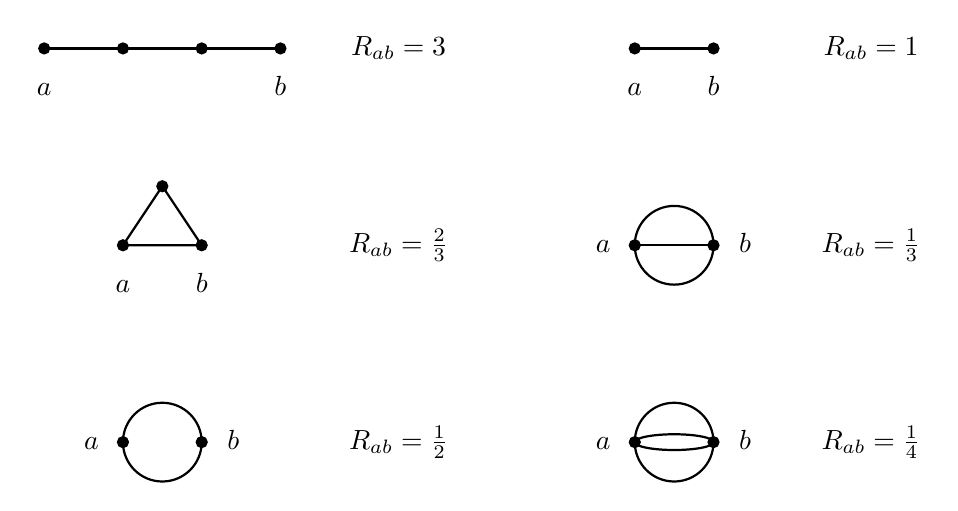
\begin{tikzpicture}

%%%3 Line segments
\begin{scope}
%Points, labels a and b
\foreach \x/\t in {-1.5/a,-.5/,.5/,1.5/b} \filldraw (\x,0) circle (2pt) node[anchor=north,yshift=-.25cm,text depth=.25ex,text height=1.5ex] {$\t$};
%Line and label R
\draw[thick] (-1.5,0) -- (1.5,0);
\node[draw=none] at (3,0) {$R_{ab}=3$};
\end{scope}

%%%Single line segment
\begin{scope}[xshift=6.5cm]
%Points, labels a and b
\foreach \x/\t in {-.5/a,.5/b} \filldraw (\x,0) circle (2pt) node[anchor=north,yshift=-.25cm,text depth=.25ex,text height=1.5ex] {$\t$};
%Line and laebl R
\draw[thick] (-.5,0) -- (.5,0);
\node[draw=none] at (2.5,0) {$R_{ab}=1$};
\end{scope}

%%%Triangle
\begin{scope}[yshift=-2.5cm]
%Points, labels a and b
\foreach \x/\y/\t in {-.5/0/a,0/.75/,.5/0/b} \filldraw (\x,\y) circle (2pt) node[anchor=north,yshift=-.25cm,text depth=.25ex,text height=1.5ex] {$\t$};
%Triangle and label R
\draw[thick] (-.5,0) -- (0,.75) -- (.5,0) -- cycle;
\node[draw=none] at (3,0) {$R_{ab}=\frac{2}{3}$};
\end{scope}

%%%Line segment and circle
\begin{scope}[xshift=6.5cm,yshift=-2.5cm]
%Points, labels a and b
\foreach \x/\t/\p/\y in {-.5/a/left/-.4,.5/b/right/.4} \filldraw (\x,0) circle (2pt) node[text depth=.25ex,text height=1.5ex] at (\x+\y,0) {$\t$};
%Line, circle, and laebl R
\draw[thick] (-.5,0) -- (.5,0);
\draw[thick] (0,0) circle (.5cm);
\node[draw=none] at (2.5,0) {$R_{ab}=\frac{1}{3}$};
\end{scope}

%%%Circle
\begin{scope}[yshift=-5cm]
%Points, labels a and b
\foreach \x/\t/\p/\y in {-.5/a/left/-.4,.5/b/right/.4} \filldraw (\x,0) circle (2pt) node[text depth=.25ex,text height=1.5ex] at (\x+\y,0) {$\t$};
%Circle and label R
\draw[thick] (0,0) circle (.5cm);
\node[draw=none] at (3,0) {$R_{ab}=\frac{1}{2}$};
\end{scope}

%%%Cross circle
\begin{scope}[xshift=6.5cm,yshift=-5cm]
%Points, labels a and b
\foreach \x/\t/\p/\y in {-.5/a/left/-.4,.5/b/right/.4} \filldraw (\x,0) circle (2pt) node[text depth=.25ex,text height=1.5ex] at (\x+\y,0) {$\t$};
%Circle, cross elipse, and label R
\draw[thick] (0,0) circle (.5cm);
\draw[thick] (0,0) ellipse (.5cm and .1cm);
\node[draw=none] at (2.5,0) {$R_{ab}=\frac{1}{4}$};
\end{scope}

\end{tikzpicture}
\caption{The effective resistance between two points for several simple graphs.
Nodes that are farther apart have a larger effective resistance, while nodes that are nearer or better connected have a smaller effective resistance.}
\label{fig:eff-res}
\end{figure}
\end{center}
%%%%%% END IMAGE %%%%%%%%

\subsection*{Link Prediction} % -----------------------------------------------

\emph{Link prediction} is the problem of predicting the likelihood of a future association between two unconnected nodes in a graph.
Link prediction has application in many fields, but the canonical example is friend suggestions on Facebook.
The Facebook network can be represented by a large graph where each user is a node, and two nodes have an edge connecting them if they are ``friends.''
Facebook aims to predict who you would like to become friends with in the future, based on who you are friends with now, as well as discover which friends you may have in real life that you have not yet connected with online.
To do this, Facebook must have some way to measure how closely two users are connected.

We will compute link prediction using effective resistance as a metric.
Effective resistance measures how closely two nodes are connected, and nodes that are closely connected at present are more likely to be connected in the future.
Given an undirected graph, the next link should connect the two unconnected nodes with the least effective resistance between them.

\begin{problem}
Write a class called \li{LinkPredictor} for performing link prediction.
Implement the \li{\_\_init\_\_()} method so that it accepts the name of a \li{csv} file containing information about a social network.
Each row of the file should contain the names of two nodes which are connected by an (undirected) edge.

Store each of the names of the nodes of the graph as an ordered list.
Next, create the adjacency matrix for the network where the $i$th row and column of the matrix correspond to the $i$th member of the list of node names.
Finally, use your function from Problem \ref{prob:effective-resistance} to compute the effective resistance matrix.
Save the list of names, the adjacency matrix, and the effective resistance matrix as attributes.
\end{problem}

\begin{problem}
Implement the following methods in the \li{LinkPredictor} class:

\begin{enumerate}
\item \li{predict\_link()}: Accept a parameter \li{node} which is either \li{None} or a string representing a node in the network. If \li{node} is \li{None}, return a tuple with the names of the nodes between which the next link should occur. However, if \li{node} is a string, return the name of the node which should be connected to \li{node} next out of all other nodes in the network. If \li{node} is not in the network, raise a \li{ValueError}. Take the following into consideration:

\begin{enumerate}
\item You want to find the two nodes which have the smallest effective resistance between them which are not yet connected.
Use information from the adjacency matrix to zero out all entries of the effective resistance matrix that represent connected nodes. The ``\li{*}" operator multiplies arrays component-wise, which may be helpful.

\item Find the next link by finding the minimum value of the array that is nonzero.
Your array may be the whole matrix or just a column if you are only considering links for a certain node.
This can be accomplished by passing \li{np.<<min>>()} a masked version of your matrix to exclude entries that are $0$.

\item NumPy's \li{np.where()} is useful for finding the minimum value in an array:

\begin{lstlisting}
>>> A = np.random.randint(-9,9,(3,3))
>>> A
array([[ 6, -8, -9],
       [-2,  1, -1],
       [ 4,  0, -3]])

# Find the minimum value in the array.
>>> minval = np.<<min>>(A)
>>> minval
-9

# Find the location of the minimum value.
>>> loc = np.where(A==minval)
>>> loc
(array([0], dtype=int64), array([2], dtype=int64))
\end{lstlisting}
\end{enumerate}


\item \li{add\_link()}: Take as input two names of nodes, and add a link between them. If either name is not in the network, raise a \li{ValueError}. Add the link by updating the adjacency matrix and the effective resistance matrix.
\end{enumerate}

Figure \ref{fig:social-network} visualizes the data in \texttt{social\_network.csv}.
Use this graph to verify that your class is suggesting plausible new links.
You should observe the following:
\begin{itemize}
\item In the entire network, Emily and Oliver are most likely to become friends next.
\item Melanie is predicted to become friends with Carol next.
\item Alan is expected to become friends with Sonia, then with Piers, and then with Abigail.
\end{itemize}
\end{problem}

\begin{figure}[H]
\includegraphics[width=.7\linewidth]{network.png}

\caption{The social network contained in \texttt{social\_network.csv}.
Adapted from data by Wayne. W Zachary (see \url{https://en.wikipedia.org/wiki/Zachary\%27s\_karate\_club}).}
\label{fig:social-network}

\begin{multicols}{4}
\begin{enumerate}
    \item Piers
    \item Abigail
    \item Oliver
    \item Stephanie
    \item Carol
    \item Melanie
    \item Stephen
    \item Sally
    \item Penelope
    \item Alan
    \item Trevor
    \item Jake
    \item Mary
    \item Anna
    \item Ruth
    \item Evan
    \item Connor
    \item John
    \item Max
    \item Eric
    \item Theresa
    \item Paul
    \item Alexander
    \item Colin
    \item Jake
    \item Jane
    \item Brandon
    \item Thomas
    \item Christopher
    \item Charles
    \item Madeleine
    \item Tracey
    \item Sonia
    \item Emily
\end{enumerate}
\end{multicols}
\end{figure}
